\section{Datahandling}
There are 12 16 bit analog digital converters (ADC) at the signal processing unit. 
Each ADC is working with 2kSPS which leads to a conversion time of $5 \cdot 10^{-4}s$. As we have 2000 samples per second the data rate of one ADC is 16 times the sample rate, which is 32kbit/s per ADC. In addition there is a total data rate of 384000 bit/s.  \\ \\
The telemetry (RS422) is requested to handle a data rate at 30kbit/s. So we are not able to send every measured value. 
To solve this problem, we  need to select the data to be send. To do this, we need to setup a frame. 
\subsection{Data frame}
\begin{figure}[htb]
	\centering
	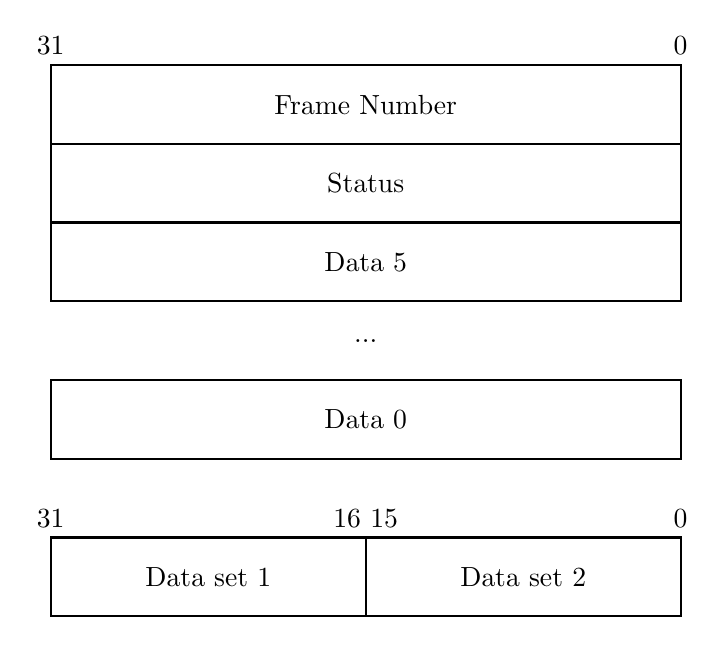
\begin{tikzpicture}
	%\draw [step=1.0,lightgray, very thin] (0.0,0.0) grid (10,10);
	% May move it 
	\draw[thick, black]  (1,10) -- (1,10) node[pos=.5,above] {31};
	\draw[thick, black]  (9,10) -- (9,10) node[pos=.5,above] {0};
	\draw[thick, black] (1, 9) rectangle (9,10) node[pos=.5] {Frame Number};
	\draw[thick, black] (1, 8) rectangle (9,9) node[pos=.5] {Status};
	\draw[thick, white] (1, 6) rectangle (9,7) node[pos=.5, black] {...};
	\draw[thick, black] (1, 7) rectangle (9,8) node[pos=.5] {Data 5};
	\draw[thick, black] (1, 5) rectangle (9,6) node[pos=.5] {Data 0};
	
	\draw[thick, black]  (1,4) -- (1,4) node[pos=.5,above] {31};
	\draw[thick, black]  (5,4) -- (5,4) node[pos=.5,above] {16 15};
	\draw[thick, black]  (9,4) -- (9,4) node[pos=.5,above] {0};
	\draw[thick, black] (1, 3) rectangle (5,4) node[pos=.5] {Data set 1};
	\draw[thick, black] (5, 3) rectangle (9,4) node[pos=.5] {Data set 2};
	\end{tikzpicture}
	\caption{Data Frame} \label{fig:sp-experimentOverview}
\end{figure} \noindent
The data frame contains a frame number, this one will be generated by the SPU software. The 32 status bit will be used to determine the current health of the system. The bits [11:0] are for the adc status bits. 0 ADC ok, 1 adc not ok. In the intervall form [14:12] will be two status bits from the MCU. All other bits are reserved. 
To handle the data with 32 bit integer values, it is necessary to transmit two values in one 32 bit value. The lower part of \ref{fig:sp-experimentOverview} shows the aligment.  \\ \\
The first three data fields (data 5 - 3) will be used to transmit the values of the strain gauges. Data 2 - 0 contains the temperature of each measurment point. The first value of the strain gauges and the first value of temeprature are from the same STAMP. So temprature two is the temperature of STAMP 2 etc.\\ \\
The header offset is 8 bytes in addtion to the 24 bytes of data one frame is about 32 bytes long. 
\subsection{Data gathering}
To gather the necessary data we have determine how many packages we are able to send at 30kbit/s. 
$$ N = \frac{30 \frac{kbit}{s}}{256 bit} = 117,18 \Rightarrow N = 116$$ 
N is the number of frame we are able to send each second. To archive this goal and reach the maximum data rating for this system we need to gather every 18th sample from each ADC. 
$$P = \frac{2000 SPS}{N} = \frac{2000 SPS}{116} = 17,24 \Rightarrow P = 18 $$
\subsection{Telemetry Source Code}
\begin{longtable}{|m{0.2\linewidth}|m{0.2\linewidth}|m{0.4\linewidth}|}
	\hline
	\textbf{Name} & \textbf{Parameter} & \textbf{Description}\\	\hline
	define NUMBEROFBYTES & - & Default value 24. Defines the data lenght in bytes. \\ \hline
	define SIZE & - & Lenght of the frame. Default 32. \\ \hline 
	typedef struct telemetry\_header\_t & uint32\_t number  uint32\_t systemstatus & [11:0] ADC error bits. [14:12] MCU Status bits. \\ \hline 
	typedef struct telemetry\_t & telemetry\_header\_t header uint8\_t data[] & Data Frame. Data lenght is defined by NUMBEROFBYTES.\\ \hline 
	telemetry\_header\_t CreateHeader & Parameter: uint32\_t stautus & Creates a header with the current number and the system status. \\ \hline 
	telemetry\_t CreatePackage & Parameter: telemetry\_header\_t *header uint8\_t *data & The pointer to the header structure and the pointer to the data. \\ \hline 
	uint32\_t SendPackage & Parameter: telemetry\_t package & Send the 32 bytes to the UART8. Casts the telemetry\_t pointer to an uint8\_t pointer. \\ \hline 
	uint32\_t PackageNumber & - & The package number \\ \hline 
	\caption{Function and structural overview}
	\label{tab:functions}
\end{longtable}